\chapter{Architecture cible}\label{chap:archi}

\section{Vue d'ensemble et couches Bronze/Silver/Gold}
L'architecture retenue est un datalake HDFS organisé en trois couches médaillon, sur le cluster Cloudera du bloc : \textbf{Bronze} (\code{chu\_bronze}) copie fidèle des extractions, un répertoire par chargement jamais modifié ; \textbf{Silver} (\code{chu\_silver}) données typées, dédoublonnées, conformées et pseudonymisées ; \textbf{Gold} (\code{chu\_gold}) constellation en étoile et vues agrégées, publiée par bascule contrôlée.

Le poste Windows porte Talend Open Studio for Big Data 7.3.1, PostgreSQL (\code{DATA2023}) et Power BI Desktop. La VM Cloudera QuickStart 5.12 porte HDFS, Hive, Hue et YARN. Talend accède au cluster par une métadonnée \emph{Cluster Hadoop} (distribution Cloudera) et des connexions HDFS et Hive.

\begin{figure}[!htbp]\centering
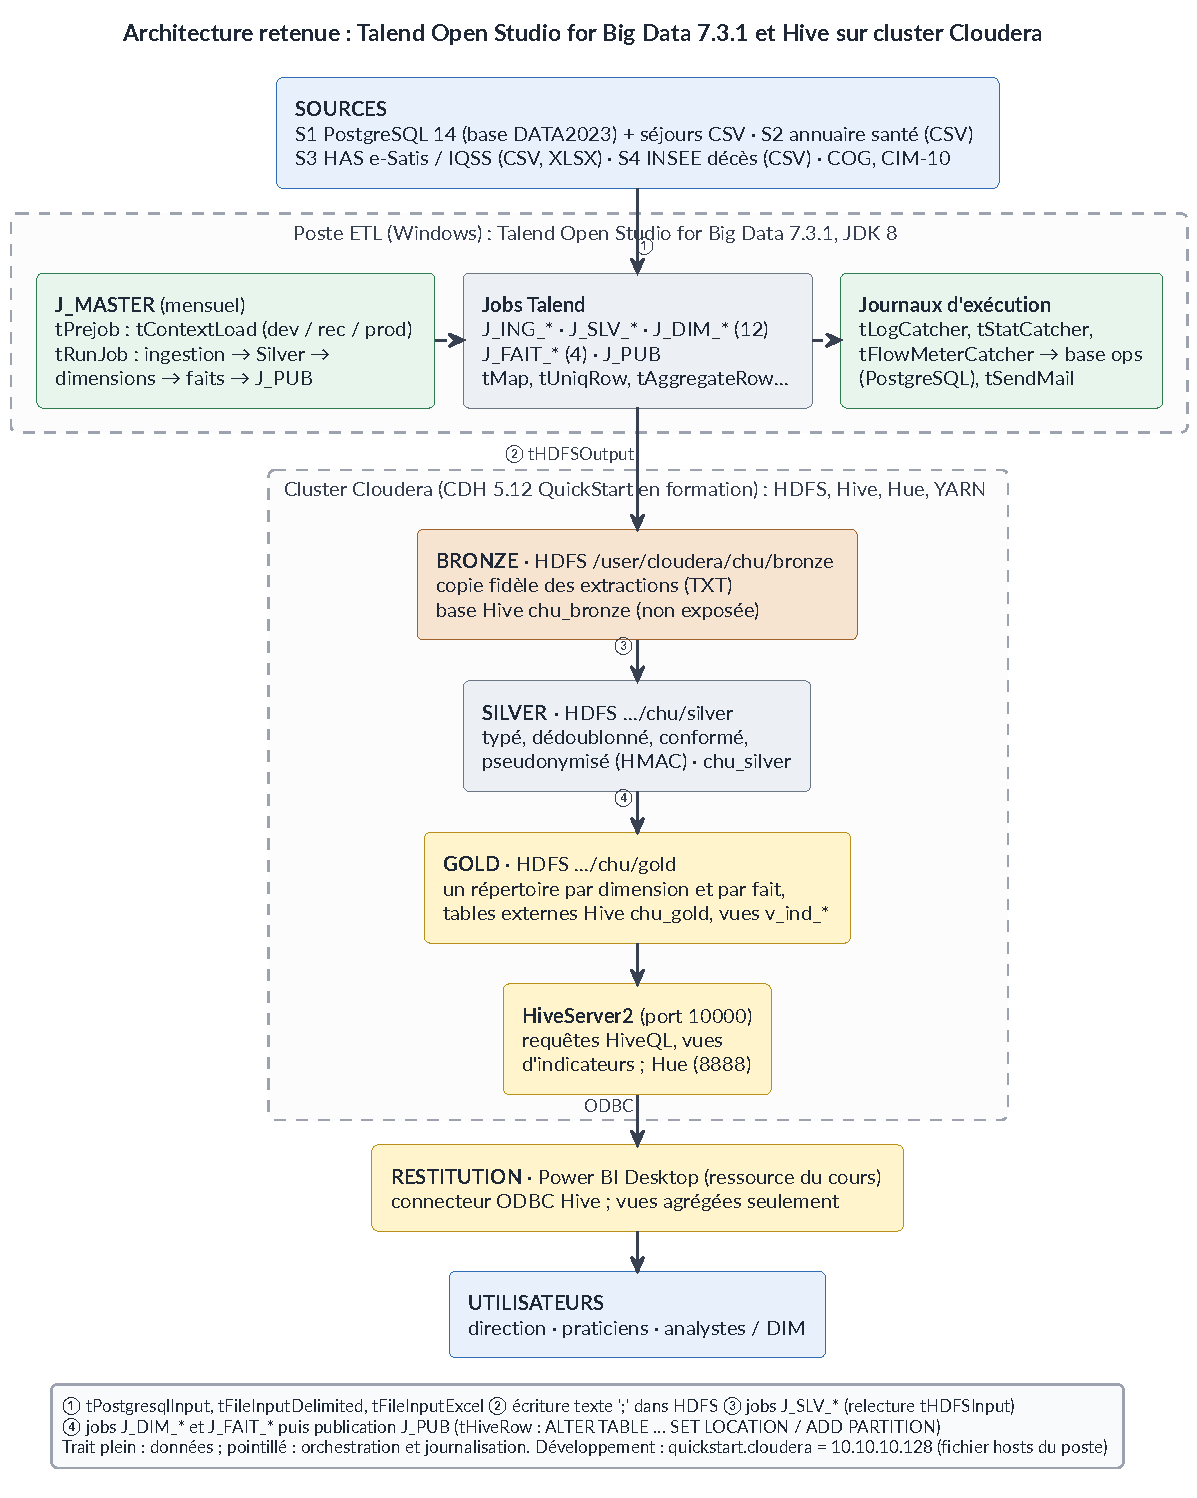
\includegraphics[width=\linewidth,height=0.6\textheight,keepaspectratio]{figures/11_architecture_globale.pdf}
\caption{Architecture retenue (jobs Talend, datalake HDFS en médaillon, tables externes Hive, Power BI)}\label{fig:archi}
\end{figure}

\section{Hiérarchie du datalake et tables Hive}\label{sec:couches}\label{sec:hierarchie}
Racine en variable de contexte (\code{hdfs\_racine}), puis couche, table, chargement mensuel :

\begin{lstlisting}[language={},frame=none,aboveskip=3pt,belowskip=3pt]
/user/cloudera/chu/                    racine = context.hdfs_racine
  bronze/ s1_patient/ s1_consultation/ s1_professionnel/ s1_diagnostic/ s1_mutuelle/
          s1_specialites/ s1_hospitalisation/ s2_etablissement/ s2_activite/
          s3_fichier/ s4_deces/ ref_cog/ ref_cim10/  (chacun : chargement=AAAAMM/)
  silver/ slv_<entite>/chargement=AAAAMM/      rejet/chargement=AAAAMM/
  gold/   dim_date/ dim_patient/ dim_sexe/ dim_tranche_age/ dim_geographie/
          dim_etablissement/ dim_diagnostic/ dim_professionnel/ dim_mutuelle/
          dim_acte/ dim_campagne/ dim_indicateur/
          fait_consultation/ fait_hospitalisation/ fait_deces/ fait_indicateur_qualite/
          (chacun : chargement=202610/  chargement=202611/  ...)
\end{lstlisting}

\textbf{Justification de la hiérarchie :}
\begin{enumerate}[nosep,leftmargin=*]
\item \textbf{Un répertoire par dimension et par fait} : une table externe Hive lit tous les fichiers de son \code{LOCATION} ; un répertoire propre à chaque table permet de charger, rejouer ou purger une dimension sans toucher aux autres.
\item \textbf{Un sous-répertoire par chargement} (\code{chargement=AAAAMM}) : le mois en cours s'écrit sans toucher au mois publié ; la publication et le retour arrière sont des bascules de métadonnées.
\item \textbf{Table externe, jamais interne} : la supprimer ne supprime pas ses fichiers ; une erreur de DDL ne détruit pas de données.
\item \textbf{Une couche par répertoire de premier niveau} : droits HDFS et base Hive par couche.
\end{enumerate}

\textbf{Format et partitionnement.} Texte délimité (\code{TEXTFILE}, \code{;}, UTF-8) : lisible par les tables externes Hive, écrit par \code{tHDFSOutput}, contrôlable dans Hue. Champ vide = \code{NULL} ; dates \code{yyyy-MM-dd}. Seuls les trois faits alimentés par ajout sont partitionnés, par \code{chargement}.

\begin{lstlisting}[style=sql,float=!htbp,label=lst:ddl,caption={Extrait du DDL HiveQL généré et publication d'un chargement}]
CREATE EXTERNAL TABLE IF NOT EXISTS dim_patient (patient_sk BIGINT,
  patient_pseudo VARCHAR(64), code_departement_residence VARCHAR(3),
  code_region_residence VARCHAR(2), id_lot VARCHAR(36), dt_chargement TIMESTAMP)
ROW FORMAT DELIMITED FIELDS TERMINATED BY ';' NULL DEFINED AS '' STORED AS TEXTFILE
LOCATION '${hivevar:racine}/gold/dim_patient/chargement=${hivevar:chargement}';
ALTER TABLE dim_patient SET LOCATION '<racine>/gold/dim_patient/chargement=202611';
ALTER TABLE fait_consultation ADD IF NOT EXISTS PARTITION (chargement='202611')
  LOCATION '<racine>/gold/fait_consultation/chargement=202611';
\end{lstlisting}

\section{Technologies retenues et justification}\label{sec:adr}
\begin{table}[!htbp]\small
\caption{Technologies retenues par brique, avec justification}\label{tab:techno}
\setlength{\tabcolsep}{4pt}
\begin{tabularx}{\linewidth}{@{}L{1.5cm}L{3.5cm}Y@{}}
\toprule\entete\textbf{Brique} & \textbf{Retenu} & \textbf{Justification}\\\midrule
ETL & \textbf{Talend Open Studio for Big Data 7.3.1} & Outil imposé par l'environnement du bloc ; composants HDFS, Hive et PostgreSQL natifs ; contextes dev/rec/prod ; \code{tMap} pour jointures et SCD~2. Alternative libre : Apache NiFi (ingestion) ou dbt (transformations SQL). \\
Stockage & \textbf{HDFS + Hive (tables externes)} & Datalake en couches sur le cluster Cloudera du bloc ; montée en charge horizontale ; tables externes sur fichiers texte. Alternative : PostgreSQL (transactions, mais un seul nœud) ou BigQuery (managé, mais hors UE). \\
BI & \textbf{Power BI Desktop} & Outil du cours ; modélisation et visuels riches ; RLS dans le service en ligne. Connexion à HiveServer2 par pilote ODBC Hive, mode \emph{Import} sur vues agrégées. Alternative : Metabase ou Apache Superset. \\
\bottomrule
\end{tabularx}
\end{table}

\textbf{Compromis acceptés.} Talend Open Studio (édition gratuite) n'est plus maintenu depuis janvier 2024 : les jobs sont exportés et versionnés, les règles de transformation sont indépendantes de l'outil. Hive en \code{TEXTFILE} n'offre ni transactions ni \code{UPDATE} : la cohérence est assurée par les répertoires de chargement et la bascule contrôlée. Power BI : le connecteur Hive natif est déprécié, d'où le pilote ODBC.

\section{Flux de données de bout en bout}\label{sec:flux}
Le job maître \code{J\_MASTER}, mensuel, enchaîne ingestion (Bronze), transformations (Silver), 12 dimensions, 4 faits et publication (figure~\ref{fig:flux}). Dimensions avant faits, portes de qualité par source.

\textbf{Publication (Write-Audit-Publish) :} chaque job Gold écrit dans \code{gold/<table>/chargement=AAAAMM/} ; \code{J\_PUB} crée une table de travail sur ce répertoire, y exécute les contrôles par \code{tHiveRow}, puis bascule par \code{SET LOCATION} (dimensions) ou \code{ADD PARTITION} (faits). En cas d'échec, rien ne bascule ; le retour arrière se fait par \code{SET LOCATION} ou \code{DROP PARTITION}.

\begin{figure}[!htbp]\centering
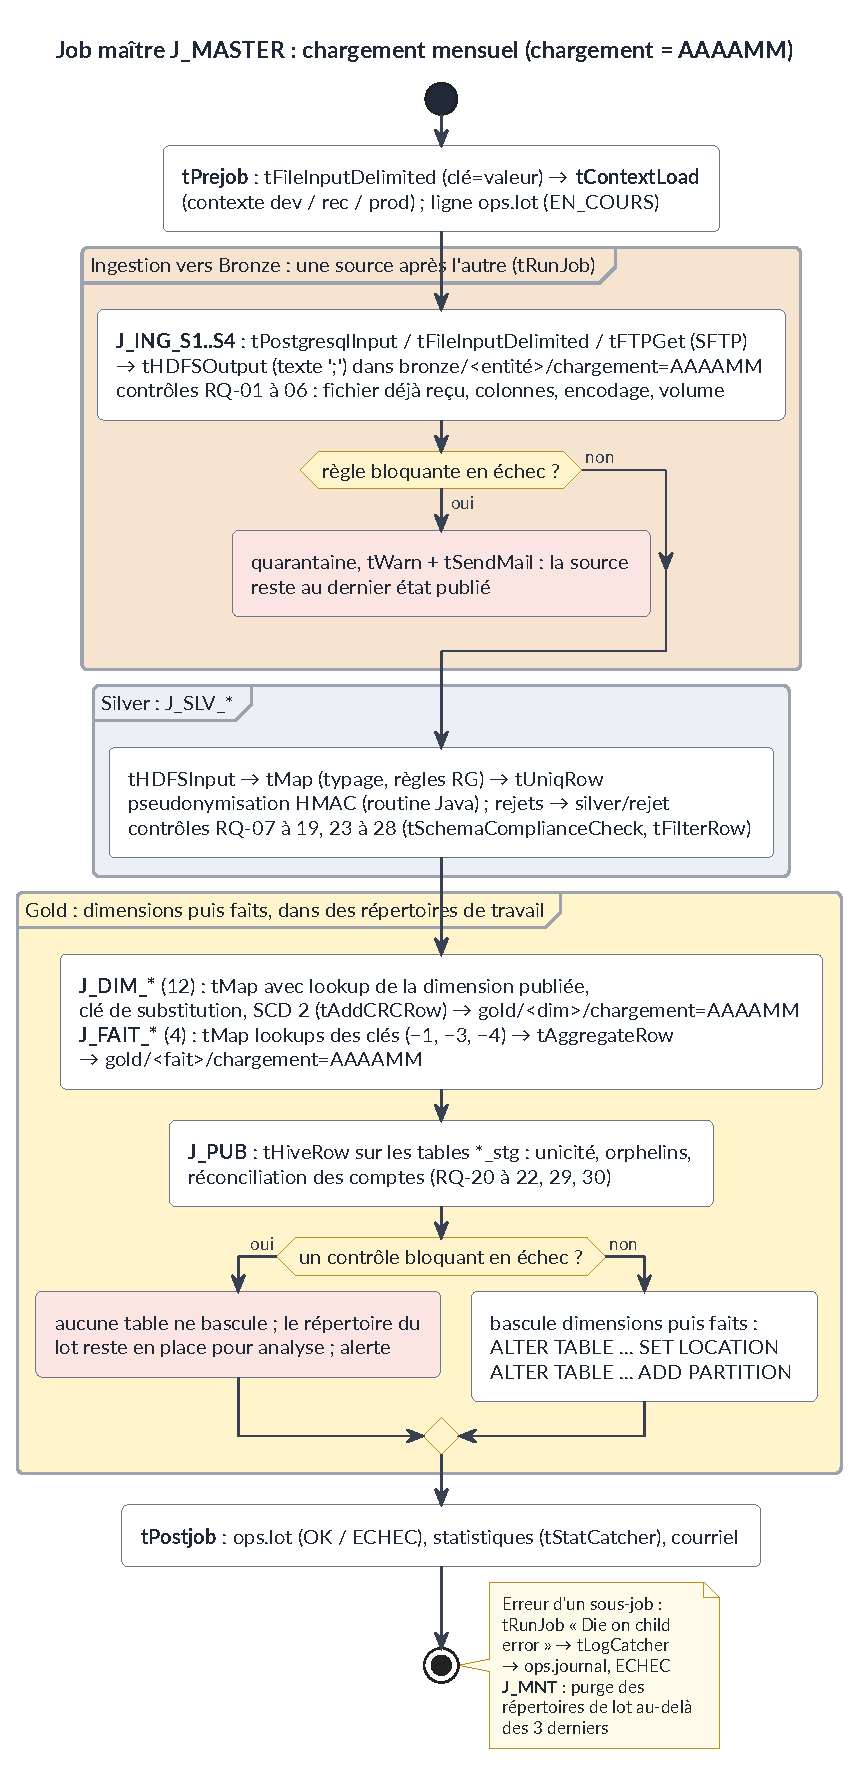
\includegraphics[width=\linewidth,height=0.66\textheight,keepaspectratio]{figures/13_flux_dag.pdf}
\caption{Job maître mensuel (portes de qualité par source, contrôles puis bascule des tables Hive)}\label{fig:flux}
\end{figure}
